%=========================================================================
% (c) 2011, 2012 Josef Lusticky

\section{Features}
Contiki OS features lightweight stackless threads called Protothreads.
Protothreads introduced a new concept to the embedded world.
They are extremely lightweight and compatible with standard C~\cite{paper-protothreads}.
Each Protothread does not require a separate stack, which fits Protothreads perfectly
for use in memory constrained embedded systems.
Protothreads are discussed in more detail in section~\ref{sec:contiki-protothreads}.

Apart from Protothreads, Contiki features a TCP/IP communication stack called uIP~(micro~IP)
that conforms to the Request For Comments memorandums published by the Internet Engineering Task Force.
The uIP stack allows Contiki to communicate over both IPv4 and IPv6~\cite{contiki-docs}.
Contiki with its uIP stack is IPv6 Ready Phase 1 certified
and therefore has the right to use the IPv6~Ready silver logo~\cite{ipv6ready-db}.
Before Contiki's uIP, the embedded world considered IP to be too heavyweight.
All previous IP implementations for general purpose computers
were much bigger than the memory constrained embedded systems could use~\cite{interconnecting}.
The uIP communication stack is further described in section~\ref{sec:contiki-uip}.

In addition to uIP, Contiki is equipped with another communication stack called Rime.
Rime is a layered communication stack for sensor networks and it uses
much thinner layers than traditional architectures~\cite{paper-rime}.
Rime is designed to simplify the implementation of communication
protocols on low-power radios.
The communication primitives in the Rime stack were chosen
based on what typical sensor network protocols use -
single-hop unicast, single-hop broadcast or multi-hop~\cite{contiki-docs,paper-rime}.

Besides Protothreads, uIP and Rime,
Contiki further contains a very simple, relatively small and easy to use filesystem
called Coffee Filesystem (CFS),
a graphical user interface Contiki Toolkit (CTK) shown in figure~\ref{fig:contiki-ctk}, an
Executable Linkable Format (ELF) loader for loading object files into a running Contiki system
and much more.

The operating system Contiki, uIP and Protothreads are used on embedded devices by hundreds of companies in
such diverse systems as car engines, oil boring equipments, satellites, and container security systems~\cite{thesis-programming}.
The software is also used in academic research
projects and in university project courses all over the world.

\begin{figure}
  \centering
  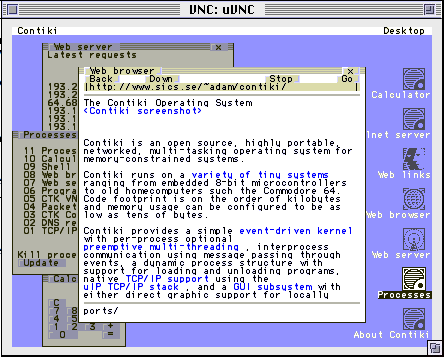
\includegraphics[width=9cm,keepaspectratio]{fig/contiki-vnc.png}
  \caption{Screenshot of running Contiki OS with CTK (source:~\cite{contiki-docs})}
  \label{fig:contiki-ctk}
\end{figure}
